\documentclass[aspectratio=169,svgnames,compress]{beamer}
% \documentclass[aspectratio=169,svgnames,compress,handout]{beamer}
\usepackage[utf8]{inputenc}
\usepackage[spanish,es-tabla]{babel}

\usepackage{graphicx} % Required for inserting images
\usepackage{tikz}
\usetikzlibrary{calc}
\usetikzlibrary{decorations.pathreplacing}
\usetikzlibrary{arrows}
\usepackage{fontawesome}
\usepackage{hyperref}
\usepackage[
    sorting=none,
    style=authoryear,
    abbreviate=true,
    eprint=false,
    url=false,
    % citepages=omit,
    % citecounter=false,
    % giveninits=true,
]{biblatex}
\usepackage{csquotes}
\usepackage[type={CC}, modifier={by}, version={4.0}]{doclicense}
\usepackage{caption}
\usepackage{subcaption}
\usepackage{fistrum}

% Cosas bibliografia
\addbibresource{references.bib}
\setbeamertemplate{bibliography item}{\faFileTextO}
\renewcommand*{\bibfont}{\footnotesize}
\DeclareCiteCommand{\footcite}%[\mkbibfootnote]
  {% \boolfalse{citetracker}%
   % \boolfalse{pagetracker}%
   \usebibmacro{prenote}%
   }
  {%
  % \ifciteindex
  %    {\indexfield{indextitle}}
  %    {}%
   \printnames[][-1]{author}
   \setunit{\adddot\space}
   % \printfield[citetitle]{labeltitle}
   \printfield{title}
   \setunit{\adddot\space}
   \printfield{year}
   \setunit{\adddot\space}
  }
  {% sepcode
    \multicitedelim%
  }
  { %postnote
  \usebibmacro{postnote}
  }

\title{Exploración de Sistemas Recomendadores para la Recomendación de Propuestas en Organizaciones Autónomas Descentralizadas}
\subtitle{Máster Universitario en Inteligencia Artificial}
\author[David Davó Laviña]{David Davó Laviña\inst{2}\\[2mm]{\footnotesize Tutores: Damiano Zanardini\inst{1} \and Javier Arroyo\inst{2}}}
\institute[UPM]{%
    \inst{1} Departamento de Inteligencia Artificial, Universidad Politécnica de Madrid \and \inst{2} Departamento de Ingeniería del Software e Inteligencia Artificial, Universidad Complutense de Madrid
}
\date{Junio 2024}

\logo{
\includegraphics[height=1cm]{images/logos/escudo-leyenda-upm-color.pdf}}
\titlegraphic{
    
\includegraphics[height=1.7cm]{images/logos/escudo-etsii-color.pdf}
    \hspace{.2cm}
    
\includegraphics[height=1.7cm]{images/logos/escudo-upm-color.pdf}
    % \hspace{.3cm}
    % \tikz\node[circle, minimum width=1.9cm,
    %     path picture = {
    %         \node at (path picture bounding box.center) {
    %             \includegraphics[width=2cm]{Images/logos/ascii.jpg}
    %         };
    %     }
    % ] {};
}

% BEAMER THEME
% \usetheme[height=1.2cm]{Rochester}

% TODO: Pass the footline option to the miniframes package
% \PassOptionsToPackage{footline=authorinstitute}{beamerouterthememiniframes}
\usetheme{Berlin}
% \usetheme{Dresden}

\usecolortheme{default}
\setbeamertemplate{navigation symbols}[only frame symbol]{}
% Only for debugging
\addtobeamertemplate{navigation symbols}{}{%
    \usebeamerfont{footline}%
    \usebeamercolor[fg]{footline}%
    \hspace{1em}%
    \insertframenumber/\inserttotalframenumber
}
% Reset the footnote number per each slide
\AtBeginEnvironment{frame}{\setcounter{footnote}{0}}

\newcommand\blfootnote[1]{
    \begingroup
    \renewcommand\thefootnote{}\footnote{#1}
    \addtocounter{footnote}{-1}
    \endgroup
}

\begin{document}

\begingroup
% DO NOT show the navigation thing in theses slides
\beamertemplatenavigationsymbolsempty
\frame[plain,noframenumbering]{\titlepage}

% \begin{frame}[allowframebreaks]{Índice}
\begin{frame}[noframenumbering]
  \frametitle{\contentsname}
  \setcounter{tocdepth}{3}

  \begin{columns}[T,onlytextwidth]
    \column{.5\linewidth}
    \tableofcontents[sections=-3]
    \column{.5\textwidth}
    \tableofcontents[sections=4-]
  \end{columns}
\end{frame}
\endgroup
\section{Introducción}

\subsection{DAOs y Blockchain}
\begin{frame}
    \begin{block}{Organización Autónoma Decentralizada (DAO)}
        Tipo de organización que permite la coordinación de proyectos mediante un proceso de \textbf{votación} democrático utilizando la tecnología \textbf{blockchain}\footnote{\textcite{hassan_decentralized_2021}}.
    \end{block}
\end{frame}

\begin{frame}
    \begin{figure}
        \centering
        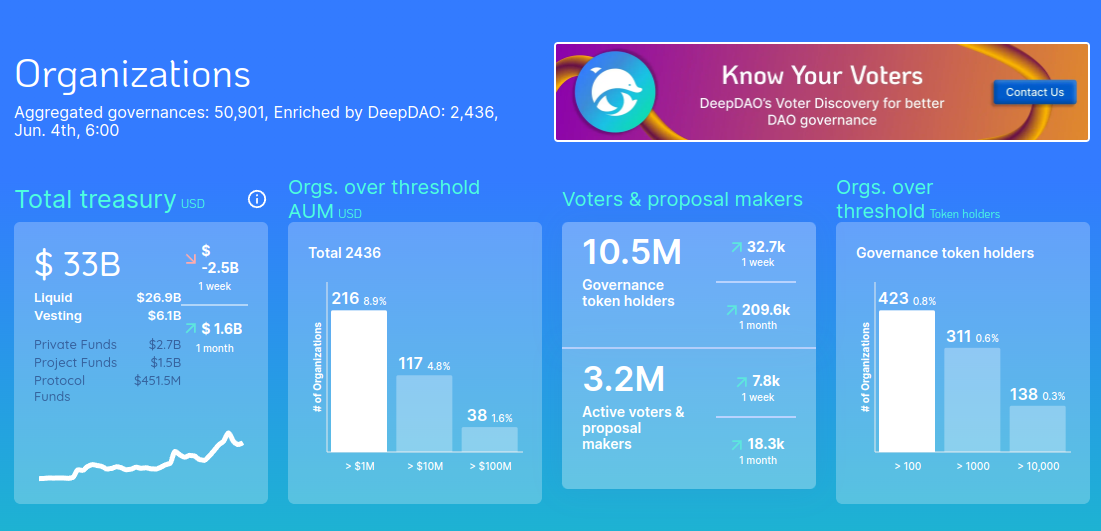
\includegraphics[height=50mm]{images/screenshots/Screenshot_20240604_172208.png}
        \caption{Captura de pantalla del portal de analíticas Deepdao\footnote{\url{https://deepdao.io/organizations}}}
        \label{fig:enter-label}
    \end{figure}
\end{frame}

\begin{frame}{Blockchain I}
    TODO: Poner una figura de ``el blockchain" (la cadena de bloques, que se vea coamo se enlazan los bloques, que tienen un hash, y poco más), y otra con como se distribuye en nodos
    % \begin{figure}
    %     \centering
    %     \includegraphics{}
    %     \caption{Caption}
    %     \label{fig:enter-label}
    % \end{figure}
\end{frame}

\begin{frame}
    \begin{figure}
        \centering
        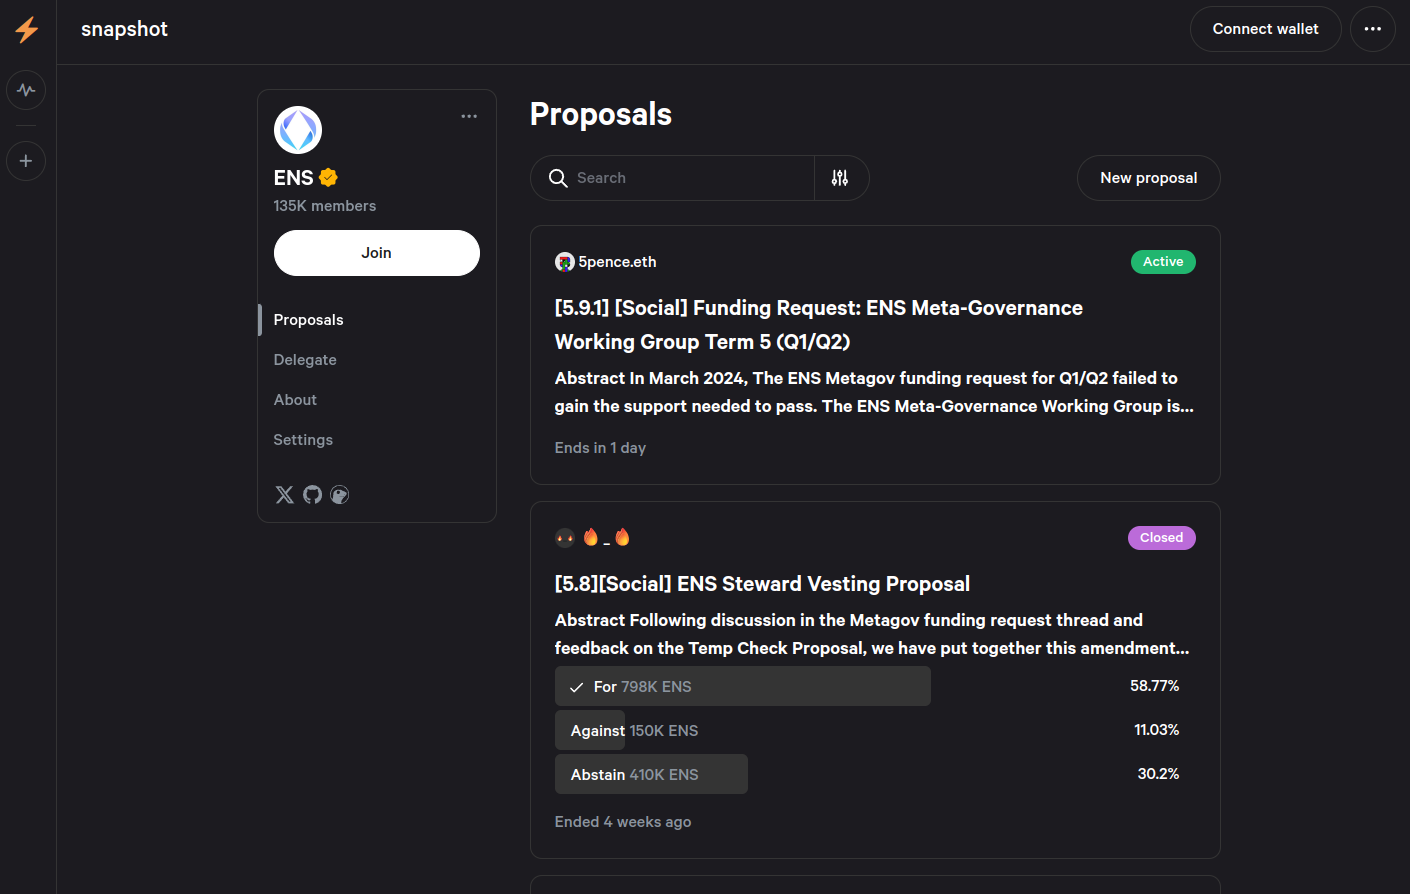
\includegraphics[width=9cm]{images/screenshots/Snapshot_ENS_Proposals.png}
        \caption{Captura de pantalla de la interfaz de votación de la DAO del protocolo ENS. \url{https://snapshot.org/\#/ens.eth}}
    \end{figure}
\end{frame}

\subsection{Motivación}

\begin{frame}
    \begin{itemize}[<+->]
        \item \textbf{Baja participación}: Menos de la mitad de usuarios han votado alguna vez\footnote{\footcite{arroyo_dao-analyzer_2022}}
        \item \textbf{Gran volumen de propuestas}: 150 propuestas/7 días en PancakeSwap o 70 en Decentraland\footnote{Notebook: \href{https://github.com/daviddavo/upm-tfm-notebooks/blob/main/04c_dao-census-onedao.ipynb}{04c\_dao-census-onedao.ipynb}}
        \item \textbf{Sin personalización}\footnote{\footcite{aviv_all_2023}}
    \end{itemize}
\end{frame}

\subsection{Sistemas Recomendadores}

\begin{frame}{DAOs y sistemas recomendadores}
    \begin{columns}
    \column{.5\textwidth}
        \begin{figure}
            \centering
            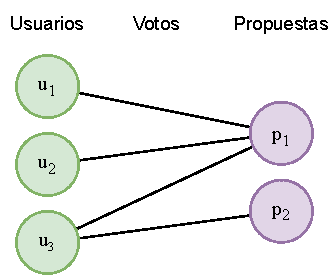
\includegraphics[height=4.5cm]{images/diagrams/dao-as-a-graph.drawio.pdf}
            \caption{Representación de una DAO como un grafo bipartito}
        \end{figure}
    \column{.5\textwidth}
        \begin{itemize}
            \item Usuarios
            \item Propuestas (\textit{ítems})
            \begin{itemize}
                \item \textbf{Descripción y texto}
                \item \textbf{Tiempo de creación}
                \item \textbf{Tiempo de cierre}
            \end{itemize}
            \item Votos (\textit{Interacción})
            \begin{itemize}
                \item \textbf{Timestamp}
            \end{itemize}
        \end{itemize}
    \end{columns}

\end{frame}

\section{Experimento}
\subsection{Conjunto de datos}

\begin{frame}{DAO census\footnote{\footcite{tfm-dataset-text}}}
\begin{columns}
\column{.35\linewidth}    
    \begin{itemize}
        \item 30~000 DAOs
        \item 5 millones de votantes
        \item 22 millones de votos emitidos
        \item 180 mil propuestas
    \end{itemize}
\column{.65\linewidth}
\pause
\begin{table}[]
    \centering
    \small
    \begin{tabular}{l|r|r|r|r}
        \textbf{DAO} & 
        \textbf{Props.} & 
        \textbf{Usu.} & 
        \textbf{Vot.} &
        \textperthousand \textbf{Dns.} \\
        \hline
DEAD Foundations      & 5 591 & 3k   & 18k  & 1.83 \\ 
PancakeSwap           & 2 691 & 130k & 533k & 3.05 \\
\textit{Decentraland} & 2 060 & 7k   & 117k & 15.47 \\
AAVE                  & 1 140 & 87k  & 2.3M & 47.28 \\
MetaCartel            &   934 & 200  & 3k   & 35.38 \\
    \end{tabular}
    \caption{Resumen de datos de algunas DAOs}
    \label{tab:my_label}
\end{table}
\end{columns}
\end{frame}

\begin{frame}{Decentraland}
\blfootnote{Fuente: Figuras 4.3 a 4.6 de la memoria}

\begin{itemize}
    \item El 50\% de los 7k usuarios han votado como mucho en 3 propuestas
    \item Las propuestas duran 7 o 14 días
    \item Media de 56 votos por propuesta
    \item Picos de hasta 70 propuestas
    \item Se suelen votar poco después (48 horas) de su fecha de creación
    \item Las propuestas no se crean uniformemente a lo largo del dia de la semana
\end{itemize}
\end{frame}

\subsection{Entrenamiento y validación}

\begin{frame}{División en entrenamiento y prueba}
    \begin{figure}
        \centering
        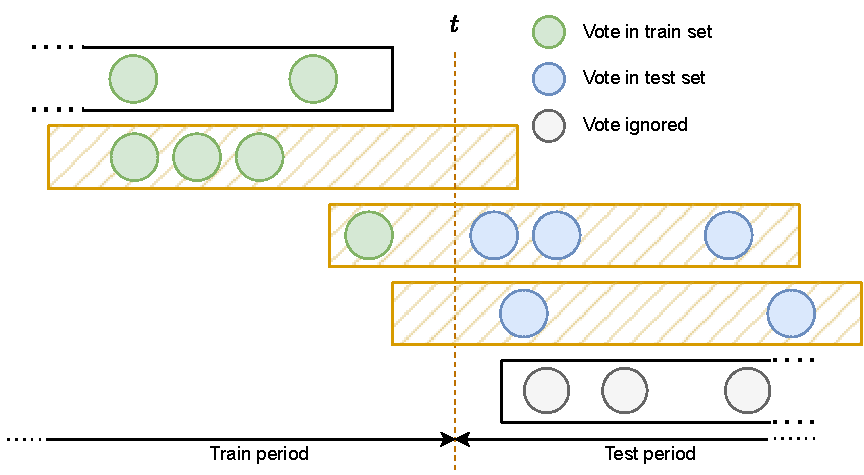
\includegraphics[height=55mm]{images/diagrams/rs-time-folds-evaluacion.drawio.pdf}
        % \caption{Ejemplo de split en \textit{entrenamiento} y \textit{prueba}}
    \end{figure}
\end{frame}


\begin{frame}{Métricas utilizadas}   
\begin{columns}
\column{.4\linewidth}
    \begin{itemize}
        \item precision@k
        \item recall@k
        \item nDCG@k
        \item MAP@k
    \end{itemize}
\column{.6\linewidth}
    \pause
    \centering
    \begin{alertblock}{Cuidado con $k>\left|\text{items rel. en top k}\right|$}
    \begin{equation}
        precision@k=\frac{\left|\text{items rel. en top k}\right|}{k}
    \end{equation}
    \end{alertblock}
\end{columns}
\end{frame}

\begin{frame}{La línea base \textit{OpenPop}}
\begin{columns}
    \column{.5\linewidth}
    \begin{alertblock}{Most Popular no tiene en cuenta:}
    \begin{itemize}
        \item La popularidad en ese momento dado
        \item Si el ítem estaba disponible
        \item Que la prop. puede estar cerrada
    \end{itemize}
    \end{alertblock}
    \column{.5\linewidth}
    \pause
    \begin{exampleblock}{OpenPop}
        Dado un instante $t$, recomendar la propuesta \textbf{abierta} más votada en ese momento siempre que el usuario no haya votado ya en ella.
    \end{exampleblock}
\end{columns}

\blfootnote{\footcite{rendle_difficulty_2019}}
\blfootnote{\footcite{ji_re-visit_2020}}
\end{frame}

\section{Modelos}
\begin{frame}
% \blfootnote{\footcite{aggarwal_recommender_2016}}
\begin{itemize}
    \item<1-> \textbf{Basado en contenido}\onslide<3->{: PLN del texto de las propuestas}
    \item<2-> \textbf{Basado en filtrado colaborativo}\onslide<3->{: Graph Neural Networks (LightGCN)}
    \item<4-> \textbf{Híbrido}: \textit{Ensemble} de los dos anteriores
    % \item<5-> \color{gray}{\textbf{Basado en conocimiento}: No hecho\footnote{\footcite{valiente_integration_2022}}}
\end{itemize}
\end{frame}

\subsection{Modelo basado en contenido}

\begin{frame}{Modelos del lenguaje}
    \begin{itemize}[<+->]
        \item Usando título y descripción de cada propuesta
        \item Python's Sentence Transformers (SBERT): \texttt{all-mpnet-base-v2} (768 dims)
        \item Importante: Utilizar tokenizador probabilístico
        \vspace*{4mm}
        \item ¿Cómo usamos los embeddings?
    \end{itemize}
\end{frame}

\begin{frame}{Ejemplo}
% DONE: Figura que muestre un ``espacio" 2d o 3d representando los embeddings de las propuestas, y ahí justo en el medio un icono del usuario
\begin{figure}
    \centering
    % Creado en parte por ChatGPT
    \begin{tikzpicture}
        % draw x and y axis
        \draw[<->, thick, color=DarkGrey] (-2,0) -- (2,0) node[anchor=north west] {};
        \draw[<->, thick, color=DarkGrey] (0,-2) -- (0,2) node[anchor=south east] {};

        % put some positive samples
        \tikzset{posprop/.style={
            fill=Green!20,
            draw=Green,
            thick,
            circle,
            minimum size=0.2cm,
            inner sep=0pt
        }}
        \node[posprop] (A) at (1,0.9) {};
        \node[posprop] (B) at (0.5,1.5) {};
        \node[posprop] (C) at (1.6,1.4) {};

        \draw<1>[->, thick, Green] ($(C.east)+(1mm,1mm)$) -- ++(6mm,2mm) node[anchor=west] {Propuesta votada};

        % put some negative samples
        \tikzset{negprop/.style={
            posprop,
            fill=Gray!20,
            draw=Gray,
        }}
        \node[negprop] at (-1,-1) {};
        \node[negprop] at (-1.2,-.6) {};
        \node[negprop] at (0.8,-.3) {};
        \node[negprop] (NA) at (-0.6,1.2) {};

        \draw<1>[->, thick, Gray] ($(NA.west)-(1mm,1mm)$) -- ++(-6mm,-2mm) node[anchor=east] {Propuesta ignorada};

        \pause
        % now the user
        \coordinate (mean) at (barycentric cs:A=1,B=1,C=1);
        \node[SkyBlue, anchor=center] at (mean) {\faUser};
        \draw<2>[->, thick, SkyBlue] ($(mean.south east)+(2mm,-2mm)$) -- ++(6mm,-3mm) node[anchor=west] {$\mu$};

        \pause
        \tikzset{newprop/.style={
            posprop,
            fill=Orange!20,
            draw=Orange,
        }}
        \node[newprop] (NP) at (1.2,1.7) {};
        \node[newprop] at (0.3,0.6) {};
        \draw<3>[->, thick, Orange] ($(NP.north)+(0mm,1mm)$) -- ++(0mm,4mm) node[anchor=south] {Nueva propuesta};

        % Force "finishing" the picture even on the first slide
        % https://tex.stackexchange.com/a/70051/107093
        \onslide<1->
    \end{tikzpicture}
    \caption{Representación simplificada del espacio latente del texto de las propuestas de un usuario}
\end{figure}
\end{frame}

\begin{frame}{Fine-tuning del PLN}
    \begin{figure}
        \centering
        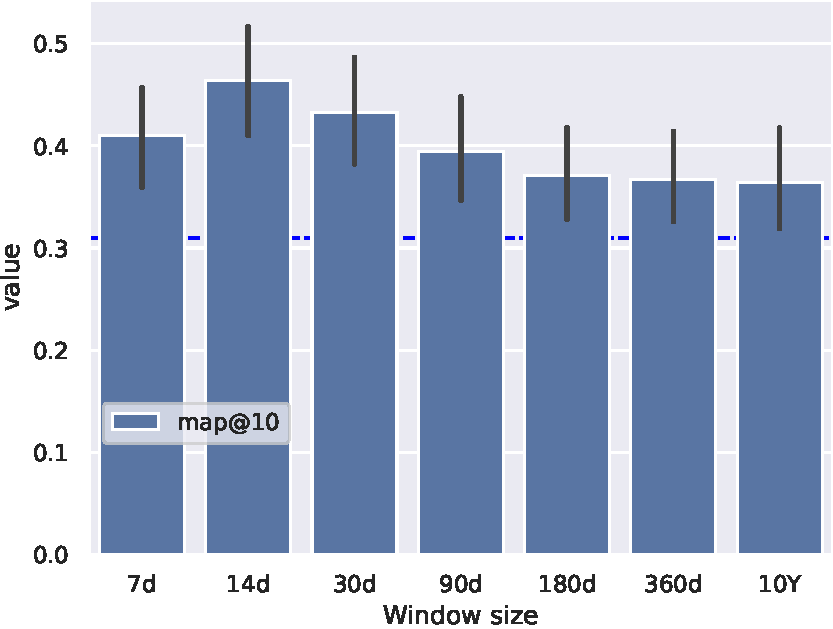
\includegraphics[height=45mm]{./images/graphs/11_cosine_results_window-size_W-THU_normalize=True_beamer.pdf}
        \caption{Rendimiento del modelo PLN con respecto al número de días utilizados para crear el modelo del usuario}
    \end{figure}
\end{frame}

\subsection{Modelo basado en filtrado colaborativo}

\begin{frame}{Graph Neural Networks}
    \begin{itemize}[<+->]
        \item SOTA en Sistemas Recomendadores
        \item Grafo Bipartito \textrightarrow\ Link prediction
        \item Nodo \textrightarrow\ Embedding
    \end{itemize}
\end{frame}

\begin{frame}{LightGCN}
    % TODO: ¿Pongo la formula de los embeddings y la agregación? Yo creo que sí, la figura del paper también tá chula.
    \footnotesize
    \vspace{-3pt}
    \begin{columns}
        \column{.5\linewidth}
        \begin{figure}
            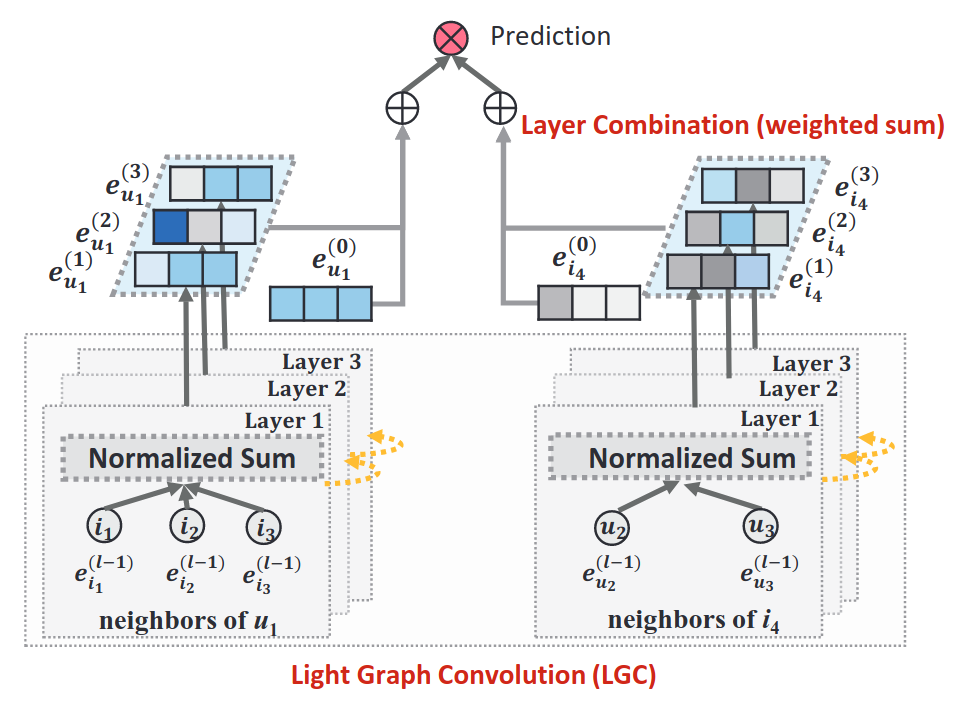
\includegraphics[width=.95\linewidth]{./images/screenshots/lightgcn_fig2.png}
        \end{figure}
        \column{.5\linewidth}
        \begin{exampleblock}{Light Graph Convolution}
            \vspace{-2pt}
            $$ 
            {\color{DarkOrange}e_u^{(k+1)}} = 
            \sum_{i\in \mathcal{N}} \frac{1}{
                \sqrt{\left|\mathcal{N}_u\right|}
                \sqrt{\left|\mathcal{N}_i\right|}
            }
            {\color{RoyalBlue}e_{i}^{(k)}}
            $$
            \vspace{-2pt}
        \end{exampleblock}
        \pause
        \begin{exampleblock}{Embedding final}
            \vspace{-2pt}
            $$ 
            {\color{DarkOrange}e_u} = \sum_{k=0}^K {\color{DarkOrange}e_u^{(k)}};\;
            {\color{RoyalBlue}e_i} = \sum_{k=0}^K {\color{RoyalBlue}e_i^{(k)}}
            $$
            \vspace{-2pt}
        \end{exampleblock}
    \end{columns}
    \blfootnote{\footcite{he_lightgcn_2020}}
\end{frame}

\begin{frame}{Fine-tuning de LightGCN I}
\begin{table}[]
    \centering
    \begin{tabular}{l|c|c}
\textbf{Hiperparámetro} & \textbf{Valores} & \textbf{Muestreo} \\
\hline
Embedding dim. & $1\leq e\leq 1024, e\in \mathbb{N}$ & Loguniforme \\
Convolution layers & $c\in \{1,2,3,4,5,6\}$ & Uniforme \\
Batch size & $bs\in\{64,128,256,512,1024\}$ & Uniforme \\
Learning rate & $10^{-4}\leq lr\leq 1, lr\in \mathbb{R}$ & Loguniforme \\
L2 regularization & $10^{-7}\leq l2 \leq 10^{-2}, l2 \in \mathbb{R}$ & Loguniforme \\
    \end{tabular}
    \caption{Espacio de búsqueda de hiperparámetros para LightGCN}
\end{table}
\blfootnote{\footcite{bergstra_making_2013}}
\blfootnote{\footcite{liaw_tune_2018}}
\end{frame}

\begin{frame}{Fine-tuning de LightGCN II}
    % Aquí pondre como una especie de ``progress bar" que se rellene con distintos colores para indicar la parte que se usa para elegir los hiperparámetros y la que se testea como ``modelo realista''
    \begin{figure}
        \centering
        \begin{tikzpicture}
            \def\trainw{3.3cm}
            \def\testw{.7cm}
            \def\recth{0.5cm}
            \def\rectspace{0.25cm}

            % Draw the four main rectangles (train and test)
            \pgfmathsetlengthmacro{\lastybot}{-4*(\recth+\rectspace)}
            \pgfmathsetlengthmacro{\bestybot}{-1*(\recth+\rectspace)}
            \foreach \i/\v in {0/0.21,1/0.34,2/0.25,3/0.17} {
                \pgfmathsetlengthmacro{\ybot}{(-\i*(\recth + \rectspace))}
                \pgfmathsetlengthmacro{\ytop}{\ybot-\recth}

                \draw[
                    thick,
                    fill=Green!20,
                    draw=Green
                ]
                    (0,\ybot)
                    rectangle
                    (\trainw,\ytop);
                \node[anchor=east] at (0,\ybot-\recth/2) {$H_\i$};
                \draw[
                    thick,
                    fill=RoyalBlue!20,
                    draw=RoyalBlue,
                ] 
                (\trainw,\ybot)
                rectangle
                (\trainw+\testw,\ytop)
                node[midway,right=3mm] (val\i) {\v};
            }

            % Draw the braces
            \draw[
                decorate,
                decoration={brace,amplitude=10pt,raise=5pt},
            ]
            (0,0) -- (\trainw,0)
            node[anchor=south,midway,above=15pt] {Entrenamiento};
            \draw[
                decorate,
                decoration={brace,amplitude=10pt,mirror},
            ]
            (0,\lastybot) -- (\trainw+\testw,\lastybot)
            node[anchor=north,midway,below=7pt] {Fold $n$};

            \pause
            % Draw the arrow
            \draw[
                -stealth,
            ] (val1.east) to ++(10mm,0) node [right] (nextfold) {$H_1$};

            % Draw the right rectangle
            \draw[
                thick,
                fill=Green!20,
                draw=Green,
            ]
            (nextfold.south east) rectangle ++(\trainw+1cm,\recth) node (nextfoldt) {};
            \draw[
                thick,
                fill=RoyalBlue!20,
                draw=RoyalBlue,
            ] (nextfoldt) rectangle ++(\testw,-\recth) node (nextfoldf) {};

            % Draw the next brace
            \draw[
                decorate,
                decoration={brace,amplitude=10pt,mirror},
            ]
            ($(nextfold.south east)+(0,-\rectspace)$) -- ($(nextfoldf)+(0,-\rectspace)$)
            node[anchor=north,midway,below=7pt] {Fold $n+1$};

            % Force "finishing" the picture even on the first slide
            % https://tex.stackexchange.com/a/70051/107093
            \onslide<1->
        \end{tikzpicture}
    \end{figure}
\end{frame}

\begin{frame}{Resultados GNN}
\begin{columns}
\column{.5\linewidth}
\begin{figure}
    \centering
    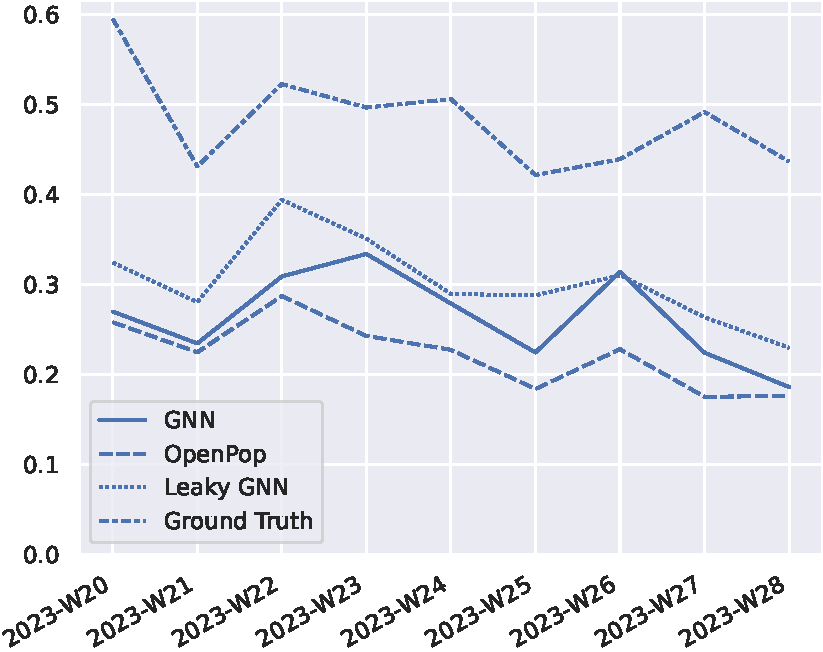
\includegraphics[height=45mm]{./images/graphs/09_gnn_results_precision_5_leaky.pdf}
    \caption{precision@5 del modelo GNN}
\end{figure}
\column{.5\linewidth}
\begin{figure}
    \centering
    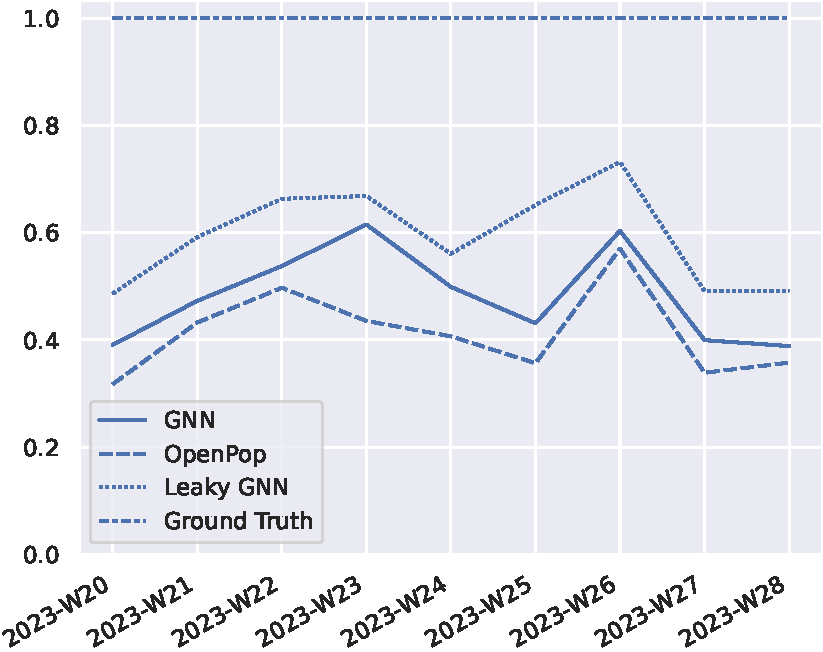
\includegraphics[height=45mm]{./images/graphs/09_gnn_results_ndcg_10_leaky.pdf}
    \caption{ndcg@10 del modelo GNN}
\end{figure}
\end{columns}
\end{frame}

\subsection{Modelo híbrido}
\begin{frame}{Comparación recomendaciones}
    \begin{figure}
        \centering
        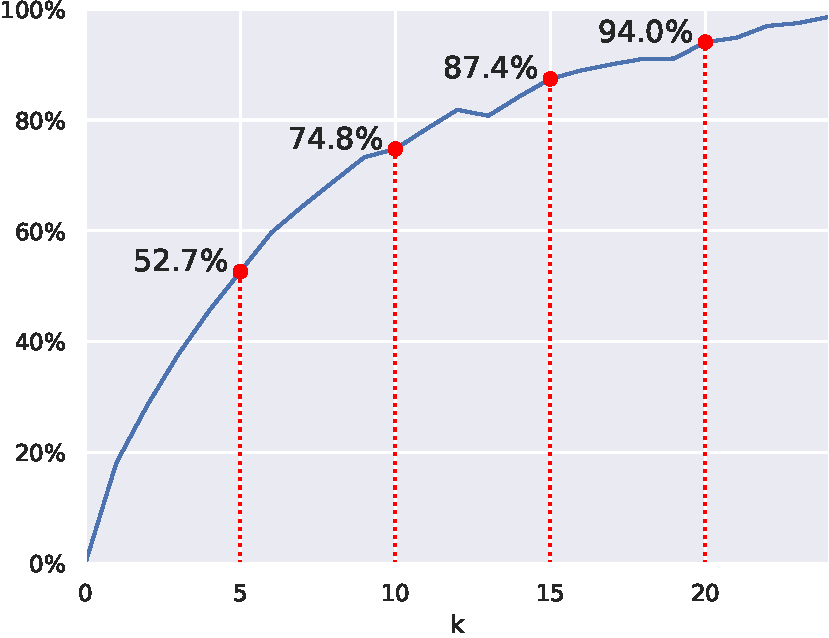
\includegraphics[height=45mm]{./images/graphs/12_hybrid_common_Decentraland_W-THU_normalize=True.pdf}
        \caption{Porcentaje de propuestas en común entre los dos recomendadores}
    \end{figure}
\end{frame}    

\begin{frame}{Métodos de fusión}
    \begin{figure}
        \centering
        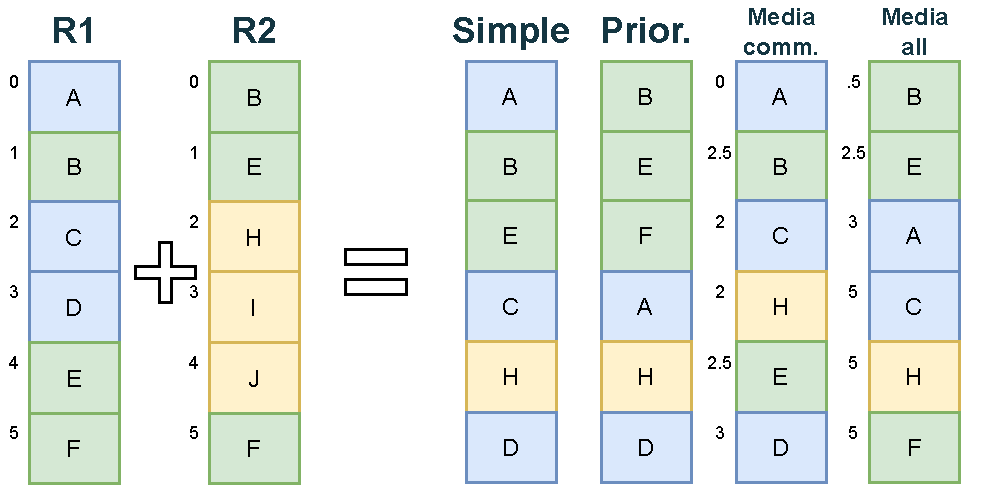
\includegraphics[height=45mm]{./images/diagrams/metodos-fusion.drawio.pdf}
        \caption{Distintos métodos de fusión utilizados}
    \end{figure}
\end{frame}

\section{Resultados}
\begin{itemize}
    \item 
\end{itemize}
\section{Conclusiones}

\begin{frame}{Trabajo realizado}
    \begin{itemize}
        \item Dataset
        \item Línea base: \textit{OpenPop}
        \item Evaluación: división en entrenamiento y prueba
        \item Desarrollo de modelos
        \item Elección de hiperparámetros
    \end{itemize}
\end{frame}

\begin{frame}{Limitaciones}
    \begin{itemize}
        \item Evaluación offline \textrightarrow ¿Cómo se comportará en realidad?
        \item Modelo GNN re-entrenado cada fold
        \item Simulación discretizada
    \end{itemize} 
\end{frame}

\begin{frame}{Trabajo futuro}
    \begin{itemize}
        \item Exploración de otros modelos
        \item Tener en cuenta el tiempo
        \item Expandir el grafo utilizado
        \item Evitar re-entrenamiento
        \item Mejorar la evaluación
        \item Probar otras maneras de elegir hiperparámetros
    \end{itemize}
\end{frame}

\begingroup
\setbeamertemplate{logo}{}
\begin{frame}{Preguntas}
    \vfill
    \begin{itemize}
        \item Código: \faGithub\ \href{https://github.com/daviddavo/upm-tfm-notebooks}{daviddavo/upm-tfm-notebooks}
        \item Diapositivas: \faGithub\ \href{https://github.com/daviddavo/upm-tfm-presentacion}{daviddavo/upm-tfm-presentacion}
    \end{itemize}
    \vfill
    \vspace{25mm}
    \doclicenseThis
\end{frame}
\endgroup

\begingroup
\beamertemplatenavigationsymbolsempty
\begin{frame}[allowframebreaks,noframenumbering]{Referencias}
    % \nocite{*}
    % \bibliographystyle{plain}
    % \bibliographystyle{acm}
    \setlength\bibitemsep{0.5\baselineskip}
    \printbibliography
\end{frame}
\endgroup

\end{document}
